\section{Introduction} \label{sec:introduction}
    \IEEEPARstart{M}{otion} modelling is a \gls{MC} technique which has shown good promise when applied to modalities such as \gls{CT}~\cite{Li2007EnhancedModel}, \gls{MR}~\cite{Manke2002RespiratoryModels} and even combined \gls{PET}/\gls{MR}~\cite{Manber2016JointCorrection.} but has not yet seen wide spread adoption in clinical \gls{PET} where \gls{PET}/\gls{CT} is far more common. \glss{MM} attempt to improve upon solely registering the data by being more robust to noise but also by allowing for the correction of unseen data. To do this \glss{MM} constrain the result of, for instance, a number of registrations to the same reference position by fitting against a \gls{SS} which allows for the parametarisation of the anatomical positional relationship of the data~\cite{McClelland2013}.
    
    \gls{RM} reduces resolution and degrades the accuracy of quantification in \gls{PET} by introducing blurring to the \gls{PET} volume and also misalignment between the \gls{PET} and \gls{CT}~\cite{Nehmeh2008a}. Most existing \gls{MC} methods rely on pair-wise registration of gated \gls{PET} volumes, this is a challenging problem due to the low contrast (uncertainty in the reconstruction) and high noise (lack of scatter correction) of these volumes~\cite{Oliveira2014}. \gls{RMC} is an ideal problem area for the application of \glss{MM} as \glss{SS} are already commonly available from respiratory gating, such as acquired by \gls{RPM} or \gls{PCA}~\cite{Thielemans2011}.
    
    In previous work the possibility of using \glss{MM} to \gls{MC} \gls{NAC} \gls{TOF} \gls{PET} data was investigated, it was found that the combination of both the \gls{MM} and \gls{TOF} data was sufficient under these circumstances~\cite{Whitehead2019ImpactPET}. Further work examined the possibility of extending this method to incorporate warping a \gls{Mu-Map} from a position close to the mean respiratory position to each gate using the \gls{MM}, it was also found here that the method was sufficient to then perform a \gls{AC} reconstruction without introducing artefacts. This work seeks to extend the method further through the use of a more modular framework which allows for the fair comparison of different registration methods, both with and without \glss{MM}. Furthermore, this work seeks to demonstrate the advantage provided by using a \gls{MM} when the count rate of the data is extremely low, where traditional registration methods would fail, and also with both scatter and random counts included (which previously was not examined, but would be evident in clinical data). Additionally, this work strives to improve the \gls{Mu-Map} warping aspect of the previous method by fixing the \gls{Mu-Map} at end inhalation, as opposed to the mean respiratory position. This is more realistic due to the vast majority of clinical \glss{Mu-Map} being a breath hold, which are further from the mean respiratory position and as such more difficult to register to.

\vspace{-0.4cm}

\section{Methods} \label{sec:methods}
    \vspace{-0.25cm}
    
    \subsection{XCAT Volume Generation} \label{sec:xcat_volume_generation}
        \gls{XCAT}~\cite{Segars2010} was used to generate $240$ volumes over a \SI{120}{\second} respiratory trace (with inter- and intra-respiratory cycle variation) derived from \gls{MR} navigator data. The max displacement of \gls{AP} and \gls{SI} motion was set to \SI{1.2}{\centi\metre} and \SI{2.0}{\centi\metre} respectively. Activity concentrations were derived from a static \gls{FDG} patient scan. The \gls{FOV} included the base of the lungs, diaphragm and the top of the liver with a \SI{20}{\milli\metre} diameter spherical lesion placed into the centre of the right lung.
    
    \vspace{-0.4cm}
    
    \subsection{PET Acquisition Simulation and Non-Attenuation Corrected Image Reconstruction} \label{sec:pet_acquisition_simulation_and_non_attenuation_corrected_image_reconstruction}
        \gls{PET} acquisitions were simulated (and reconstructed) using \gls{STIR}~\cite{Thielemans2012, Nikos2019} through \gls{SIRF}~\cite{Ovtchinnikov2017} to forward project the data using the geometry of a \gls{GE} Discovery $710$ with a \gls{TOF} resolution of \SI{375}{\pico\second}. This \gls{TOF} resolution is higher than that of the $710$, but is closer to the newer \gls{GE} Signa \gls{PET}/\gls{MR} system. \gls{TOF} mashing was used to reduce computation time resulting in $13$ \gls{TOF} bins of size \SI{376.5}{\pico\second}. Attenuation was included using the relevant \glss{Mu-Map} generated by \gls{XCAT}.
        
        Randoms were added by summing the scaled mean value to each voxel of each volume prior to forward projection. Pseudo scatter was added by summing the scaled and smoothed mean \gls{Mu-Map} prior to forward projection, the smoothing parameter was optimised to give scatter which tapered at the same rate as in clinical data. A full scatter simulation was not performed due to software limitations.
        
        Multiple noise realisations were generated to simulate an acquisition over \SI{120}{\second}, emulating a standard single bed position acquisition. The count rate was selected to match that of research scans, in other words, the count rate was below that of diagnostic clinical scans. This count rate was selected as a 'worst case scenario'.
        
        A respiratory \gls{SS} was generated using \gls{PCA}~\cite{Thielemans2011}. This was used to gate the data into $10$ respiratory bins using displacement gating. For the purpose of the \gls{MM} fitting, \gls{SS} values were determined for the post-gated data by taking an average of the \gls{SS} values of the data in each bin.
        
        Data were reconstructed without \gls{AC} using OSEM with two full iterations and $24$ subsets.~\cite{Hudson1994}.
    
    \vspace{-0.4cm}
    
    \subsection{Registration} \label{sec:registration}
        Before being registered each volume underwent pre-processing, this pre-processing was only applied to intermediate data and was not apparent in the output of the method. Initially, because a breath hold \gls{Mu-Map} is the final target position for the \gls{MC} $10$ repeating slices are added to the top and bottom of each volume to allow space for the volumes to be registered into. First, the mean value was subtracted from each volume and then each voxel in the volume was divided by the standard deviation of the volume. Next a Yeo-Johnson transformation~\cite{Johnson2013} was applied to transform the data to be more Gaussian like, this acted as a pseudo histogram normalisation. Finally the data underwent Gaussian smoothing.
        
        Two registration methods were examined in this work. Firstly, pair-wise registration, where the reference position was selected as the gate with the highest number of counts and all other gates were registered to it. Secondly, group-wise registration, where after an initial pair-wise registration step the \glss{DVF} generated had the inverse mean of all \glss{DVF} composed with them before a new reference volume was resampled. Registration to the new reference volume followed by the inverse mean composition and resample continued for a set number of iterations. NiftyReg~\cite{Modat2010} was used to perform indirect registrations using a B-spline parameterisation. The \gls{CPG} spacing of the B-spline coefficients, bending energy regularisation term weight and Gaussian smoothing parameters were tuned using a grid search.
    
    \vspace{-0.4cm}
    
    \subsection{Motion Model Estimation} \label{sec:motion_model_estimation}
        If a \gls{MM} was used then it was fit as a direct \gls{RCM} on the \glss{DVF} from~\Fref{sec:registration} and the \gls{SS} from~\Fref{sec:pet_acquisition_simulation_and_non_attenuation_corrected_image_reconstruction}. A weighted \gls{LR} was used where the weighting was taken based on the number of counts in each gate. Once a \gls{MM} was fit, new \glss{DVF} were generated for each gate using the \gls{SS} values used to fit the \gls{MM}.
    
    \vspace{-0.4cm}
    
    \subsection{Attenuation Map Warping} \label{sec:attenuation_map_warping}
        A \gls{Mu-Map} at end inhalation was selected from the \glss{Mu-Map} generated by \gls{XCAT}. The \gls{PET} volume from the previous step was then registered to this \gls{Mu-Map} and the resulting \glss{DVF} were composed with the \glss{DVF} from the last iteration of the \gls{MC} method and a new volume resampled. The inverse of these \glss{DVF} were then used to warp the \gls{Mu-Map} to each gate.
    
    \vspace{-0.4cm}
    
    \subsection{Motion Corrected Image Reconstruction with AC} \label{sec:attenuation_corrected_image_reconstruction}
        Data was re-reconstructed, with \gls{AC}, using the \glss{Mu-Map} from~\Fref{sec:attenuation_map_warping}. The same reconstruction parameters as in~\Fref{sec:attenuation_corrected_image_reconstruction} were used. \gls{MC} was then applied to this data following the same steps as above. Volumes were post-filtered using a Gaussian blur with a kernel size of \SI{6.39}{\milli\metre} \gls{FWHM} in the transverse plane and \SI{3.27}{\milli\metre} \gls{FWHM} in the axial direction.
    
    \vspace{-0.4cm}
    
    \subsection{Evaluation} \label{sec:evaluation}
        In addition to the reconstructions performed in~\Fref{sec:attenuation_corrected_image_reconstruction} data was also reconstructed without \gls{MC} using either a sum of all \glss{Mu-Map} (to emulate an average CINE-CT) or the end inhilation \gls{Mu-Map}. For the sake of evaluation these volumes were registered to the position of the end inhalation \gls{Mu-Map}.
        
        Comparisons used included: A profile over the lesion and \gls{SUV}\textsubscript{max} and \gls{SUV}\textsubscript{peak} (defined following \gls{EANM} guidelines~\cite{Boellaard2015FDG2.0}).

\vspace{-0.4cm}

\section{Results} \label{sec:results}
    \begin{figure}
        \vspace{-0.4cm}
        \centering
        
        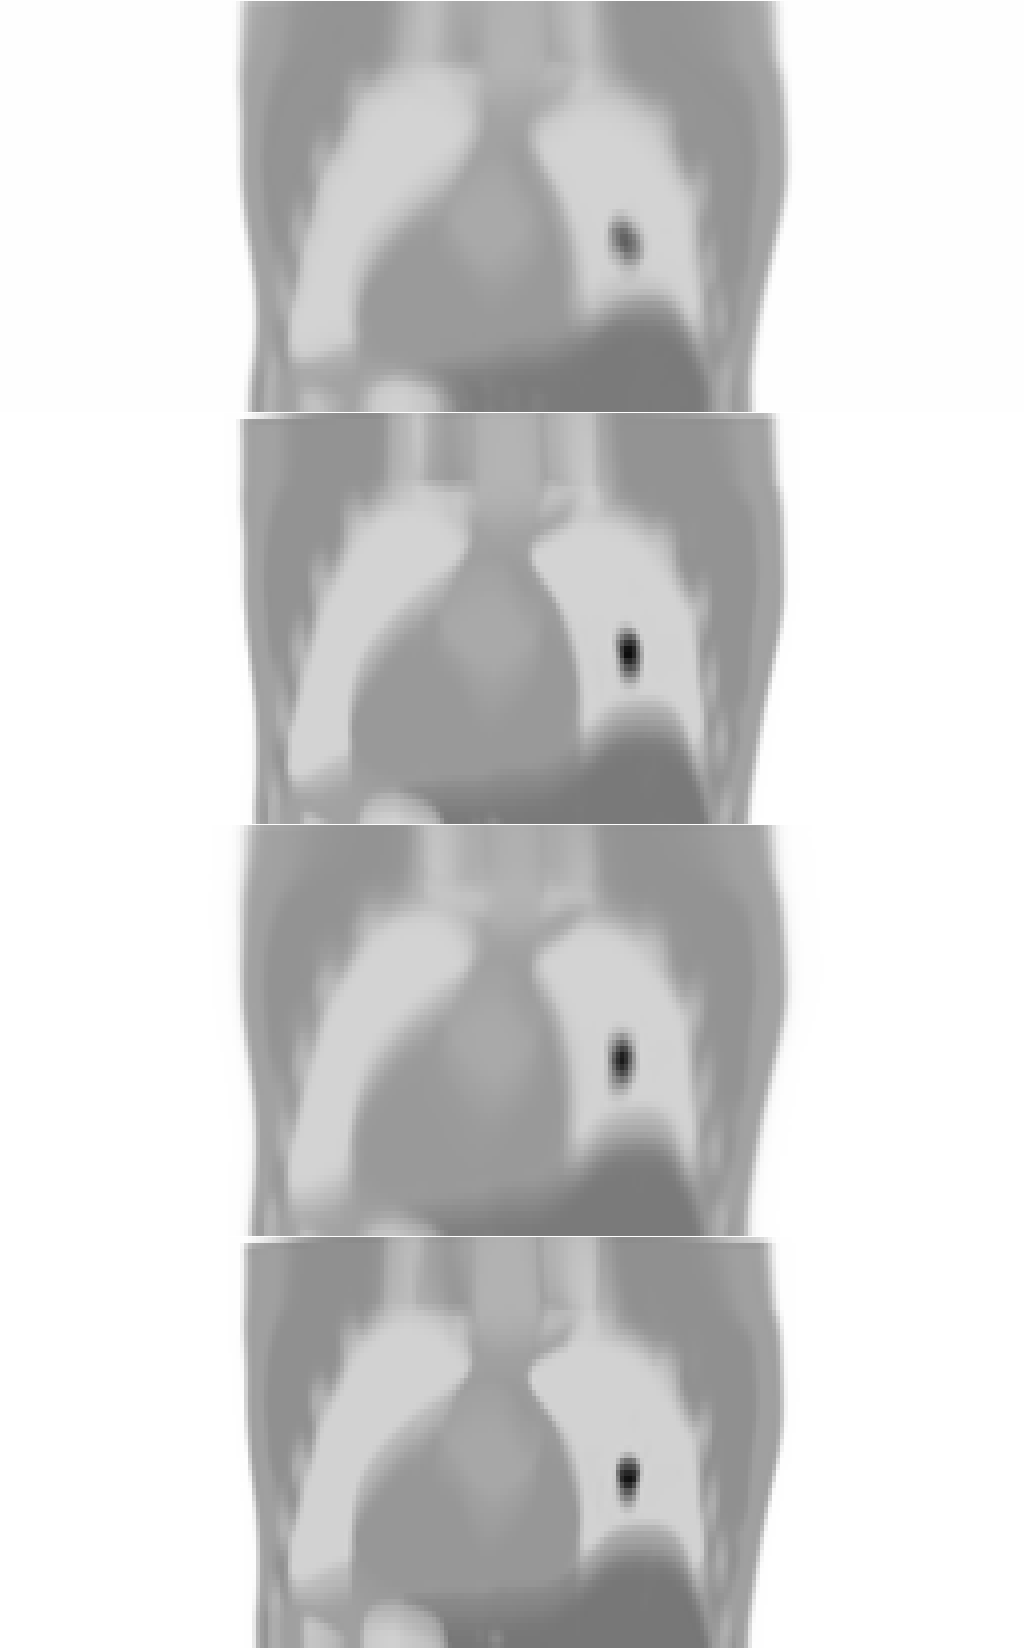
\includegraphics[width=1.0\linewidth]{figures/visual_analysis.png}
        
        \vspace{-0.4cm}
        
        \captionsetup{singlelinecheck=false, justification=centering}
        \caption{Reconstructions using; ungated (static \gls{CT}), ungated (CINE-\gls{CT}), pair-wise, pair-wise \gls{MM}, group-wise, group-wise \gls{MM}. Colour map ranges are consistent for all images.}
        
        \label{fig:visual_analysis}
        
        \vspace{-0.4cm}
    \end{figure}
    
    \begin{figure}
        \vspace{-0.4cm}
        \centering
        
        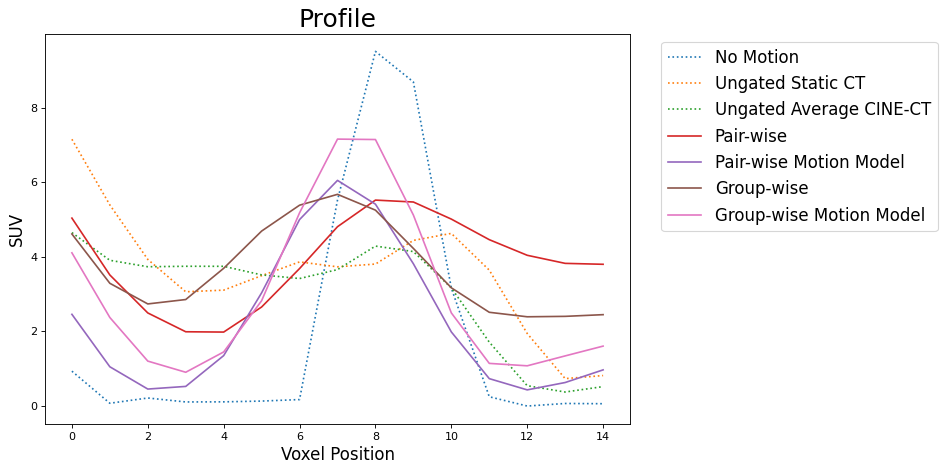
\includegraphics[width=1.0\linewidth]{figures/profile.png}
        
        \vspace{-0.4cm}
        
        \captionsetup{singlelinecheck=false, justification=centering}
        \caption{A profile across the lesion for; ungated (static \gls{CT}), ungated (CINE-\gls{CT}), pair-wise, pair-wise \gls{MM}, group-wise, group-wise \gls{MM}.}
        
        \label{fig:profile}
        \vspace{-0.4cm}
    \end{figure}
    
    \begin{table}
        \centering
        
        \captionsetup{singlelinecheck=false, justification=centering}
        \caption{Comparison of \gls{SUV}\textsubscript{max} and \gls{SUV}\textsubscript{peak} between; ungated (static \gls{CT}), ungated (CINE-\gls{CT}), pair-wise, pair-wise \gls{MM}, group-wise, group-wise \gls{MM}.}
        
        \resizebox*{0.8\linewidth}{!}
        {
            \begin{tabular}{||c|cc||}
                \hline
                \textbf{\gls{SUV}}              & \textbf{Max}  & \textbf{Peak} \\
                \hline
                \textbf{pair-wise}               & $4.35$        & $3.93$ \\
                \textbf{pair-wise Motion Model}  & $6.59$        & $5.78$ \\
                \textbf{group-wise}              & $6.27$        & $5.31$ \\
                \textbf{group-wise Motion Model} & $6.84$        & $6.40$ \\
                \hline
            \end{tabular}
        }
        
        \label{tab:suv}
        \vspace{-0.4cm}
    \end{table}
    
     A slice passing through the lesion for each method can be seen in~\Fref{fig:visual_analysis}. When compared visually more blurring can be seen at the boundary between the diaphragm and lung for the examples where a \gls{MM} wasn't used, additionally where a \gls{MM} was used the lesion appears to be more homogeneous. Furthermore, a profile passing through the lesion and diaphragm can be seen in~\Fref{fig:profile}. The peak of the profile is greater for both group-wise methods than for both pair-wise methods and each \gls{MM} example is greater than when \gls{MM} isn't used. \gls{SUV} results can be seen in~\Fref{tab:suv} and consistently show that including a \glss{MM} significantly increases the \gls{SUV} when compared to when one isn't used.

\vspace{-0.4cm}

\section{Discussion and Conclusions} \label{sec:discussion_and_conclusions}
    Results from a visual analysis, a comparison of profiles and \glss{SUV} show that adding a \gls{MM} to any \gls{MC} method, tested here, immediately improved the quality of volumes produced, not only in a way which increased visual contrast but also in a quantitative way. Furthermore, while it seemed that performing either pair-wise or group-wise registration didn't have the same impact as incorporating a \gls{MM} it appears, for the same reasons as previously, that if the added computation time required of group-wise registration is of negligible impact then it is preferable to use group-wise over pair-wise.
    
    In the future, work will focus on incorporating the methods presented here into an interative \gls{IR} and \gls{MC} method. It may also be of interest to consider the impact that robust regression methods have on fitting a \gls{MM}, such as using a robust objective function or fitting the \gls{MM} indirectly on the eigenvectors of applying \gls{PCA} to the initial \glss{DVF}.
    